\documentclass[tikz]{standalone}
\renewcommand*{\familydefault}{\sfdefault}
\usepackage{standalone}
\usepackage{amssymb}
\usetikzlibrary{decorations}
%\usetikzlibrary{arrows.meta, decorations.pathmorphing, decorations.pathreplacing, shapes.geometric}
\usetikzlibrary{bayesnet}

\begin{document}
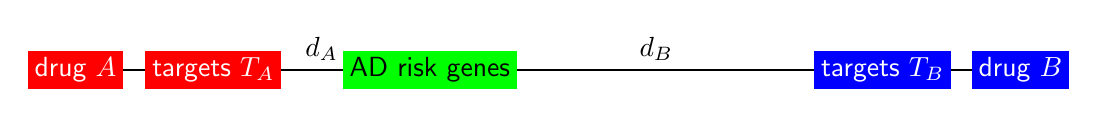
\begin{tikzpicture}
\path[draw] (0,0) node[white,rectangle,inner sep=2.5pt,fill=red] {drug $A$} --
(1.75,0) node[white,rectangle,inner sep=2.5pt,fill=red] {targets $T_A$} --
node[anchor=south]{$d_A$}
(4.5,0) node[black,rectangle,inner sep=2.5pt,fill=green] {AD risk genes} --
node[anchor=south]{$d_B$}
(10.25,0) node[white,rectangle,inner sep=2.5pt,fill=blue] {targets $T_B$} --
(12,0) node[white,rectangle,inner sep=2.5pt,fill=blue] {drug $B$};
;
\end{tikzpicture}
\end{document}
